% =====================================================================
%  ESP32-S3 Production Firmware — Corrected MQTT Sequence (EMQX best practice)
%  ETERNITY / ONEOPS Platform — companion to the Unified Technical Spec
%
%  Build:  pdflatex esp32-firmware-sequence.tex   (run twice)
%  Pure TikZ — no external sequence-diagram package required.
% =====================================================================
\documentclass[11pt,a4paper]{article}

\usepackage[utf8]{inputenc}
\usepackage[T1]{fontenc}
\usepackage[margin=2.2cm]{geometry}
\usepackage{xcolor}
\usepackage{amssymb}
\usepackage{booktabs}
\usepackage{array}
\usepackage{tabularx}
\usepackage{enumitem}
\usepackage{graphicx}
\usepackage{caption}
\usepackage{float}
\usepackage{tikz}
\usetikzlibrary{arrows.meta,calc,positioning,backgrounds,fit,shapes.misc}

% ---------------------------------------------------------------------
%  Palette
% ---------------------------------------------------------------------
\definecolor{devCol}{HTML}{2E7D32}   % ESP32 device   (green)
\definecolor{brkCol}{HTML}{6A1B9A}   % EMQX broker    (purple)
\definecolor{svcCol}{HTML}{1565C0}   % services       (blue)
\definecolor{dbCol}{HTML}{00838F}    % datastore      (teal)
\definecolor{otaCol}{HTML}{EF6C00}   % OTA / artefact (orange)
\definecolor{usrCol}{HTML}{C62828}   % operator       (red)
\definecolor{bandCol}{HTML}{ECEFF4}  % phase band
\definecolor{noteCol}{HTML}{FFF8E1}  % note fill
\definecolor{noteEdge}{HTML}{F9A825}

% ---------------------------------------------------------------------
%  Sequence-diagram engine (auto-advancing vertical cursor \YY)
% ---------------------------------------------------------------------
\newcommand{\msgstep}{0.70}
\newcommand{\seqreset}{\xdef\YY{-1.30}}
\newcommand{\adv}{\pgfmathsetmacro{\tmp}{\YY-\msgstep}\xdef\YY{\tmp}}
\newcommand{\gap}{\pgfmathsetmacro{\tmp}{\YY-0.35}\xdef\YY{\tmp}}

\tikzset{
  head/.style={draw, rounded corners=2pt, minimum width=2.05cm, minimum height=0.66cm,
               font=\footnotesize\bfseries, text=white, align=center},
  lifeline/.style={densely dashed, gray!60, line width=0.5pt},
  msg/.style={-{Stealth[length=5pt]}, line width=0.7pt},          % control packet / sync call
  evt/.style={-{Stealth[length=5pt]}, densely dashed, line width=0.7pt, brkCol}, % broker delivery / async event
  ret/.style={-{Triangle[open,length=5pt]}, densely dotted, gray, line width=0.6pt}, % return
  mlbl/.style={midway, above, font=\scriptsize, inner sep=1.4pt, align=center},
  mlblb/.style={midway, below, font=\scriptsize, inner sep=1.4pt, align=center},
  notestyle/.style={draw=noteEdge, fill=noteCol, rounded corners=1pt, font=\scriptsize,
                    align=left, inner sep=3pt, text width=#1},
  band/.style={fill=bandCol, draw=gray!40, rounded corners=2pt, font=\footnotesize\bfseries\itshape,
               text=black!75, minimum height=0.5cm, align=center},
}

% solid message:  \mO{fromX}{toX}{label}
\newcommand{\mO}[3]{\draw[msg] (#1,\YY) -- (#2,\YY) node[mlbl]{#3};\adv}
% solid message, label below (for tight return-direction lines)
\newcommand{\mOb}[3]{\draw[msg] (#1,\YY) -- (#2,\YY) node[mlblb]{#3};\adv}
% async broker delivery / event
\newcommand{\mA}[3]{\draw[evt] (#1,\YY) -- (#2,\YY) node[mlbl,text=brkCol]{#3};\adv}
% return / response
\newcommand{\mR}[3]{\draw[ret] (#1,\YY) -- (#2,\YY) node[mlbl,text=gray]{#3};\adv}
% self action:  \mS{X}{label}
\newcommand{\mS}[2]{%
  \draw[msg] (#1,\YY) -- ++(0.55,0) -- ++(0,-0.26) -- ++(-0.55,0);
  \node[anchor=west,font=\scriptsize,inner sep=1.4pt] at ([xshift=17pt,yshift=-4pt]#1,\YY){#2};
  \pgfmathsetmacro{\tmp}{\YY-0.82}\xdef\YY{\tmp}}
% note anchored at x:  \note{x}{width}{text}
\newcommand{\note}[3]{\node[notestyle=#2] at (#1,\YY){#3};\adv}
% full-width phase band centred at \xmid:  \phase{text}
\newcommand{\phase}[1]{\gap\node[band,minimum width=\bandw] at (\xmid,\YY){#1};\adv}

\newcommand{\seqtitle}[1]{\textbf{#1}}

% =====================================================================
\begin{document}

\begin{center}
  {\LARGE\bfseries ESP32-S3 Production Firmware}\\[2pt]
  {\large Corrected MQTT Sequence following EMQX Broker Best Practices}\\[6pt]
  {\small ETERNITY\,/\,ONEOPS Platform — companion to the \emph{Unified Technical Specification v1.0}}\\[2pt]
  {\small\itshape Revised 2026-06-08}
\end{center}

\vspace{4pt}
\hrule
\vspace{8pt}

\section*{1\quad Scope and what was corrected}
The specification's end-to-end sequence (\S5.6/\S5.7) begins at \texttt{publish reading}
and treats the broker as a dumb pipe. That hides the parts of the firmware contract that
actually decide field reliability: \emph{how the device authenticates, how presence is
tracked, how sessions and commands survive a flaky link, and how firmware is delivered
safely}. This document redraws the lifecycle of a single production device against
\textbf{EMQX} broker semantics (MQTT~5.0) and marks every correction.

\begin{center}
\renewcommand{\arraystretch}{1.28}
\small
\begin{tabularx}{\textwidth}{@{}p{3.0cm} p{4.6cm} X@{}}
\toprule
\textbf{Area} & \textbf{Original spec} & \textbf{Corrected — EMQX best practice} \\
\midrule
Transport \& auth & shared / implicit; ``returns mTLS cert'' but no handshake shown &
  one-time factory \emph{bootstrap} token over server-auth TLS, immediately rotated to
  \textbf{per-device X.509 client certificate}; steady state is \textbf{mutual TLS 1.3}
  verified by EMQX. \\
Client identity & ``initial \texttt{device\_id}'' &
  stable, unique \texttt{mqtt\_client\_id} bound to the certificate CN; duplicate-ID
  takeover rejected. \\
Authorization & not stated &
  EMQX \textbf{ACL}: a device may only publish/subscribe under
  \texttt{devices/\{id\}/\#} and \texttt{sensors/\{sid\}/raw}; cross-device spoofing denied. \\
Session & not stated &
  MQTT~5.0 \texttt{clean\_start=0} + \textbf{Session-Expiry}, so QoS~1 commands queued
  during a brief drop are redelivered on reconnect. \\
Presence (LWT) & \texttt{status} is ``LWT topic'', retain unspecified &
  Will published \textbf{QoS~1, retain=1}; matching \textbf{birth} message on (re)connect
  clears it, so late subscribers always read correct state. \\
Config delivery & plain publish &
  \texttt{devices/\{id\}/config} published \textbf{retain=1, QoS~1} $\Rightarrow$ device
  gets current config the instant it subscribes. \\
Heartbeat & QoS~0, retain=0 \checkmark &
  kept QoS~0; \texttt{keepalive=60\,s}, EMQX dead-peer detection at $1.5\times$ keepalive. \\
Sensor reading & QoS~1, retain=0 \checkmark &
  kept QoS~1 (PUBACK); ingest consumes via an EMQX \textbf{shared subscription}
  (\texttt{\$share/ingest/\dots}) for horizontal scale + back-pressure. \\
OTA & ``upgrade to 1.4.2 from \texttt{artefact\_uri}'' &
  \textbf{signed} artefact (SHA-256 + secure-boot), \textbf{A/B} partition, out-of-band
  HTTPS fetch, \texttt{ota/progress} telemetry, \textbf{automatic rollback}, audit row in
  \texttt{device\_firmware\_history}. \\
Abuse control & none &
  EMQX \textbf{flapping detection} + per-client message/bandwidth rate limits. \\
\bottomrule
\end{tabularx}
\end{center}

\paragraph{Legend.}
\tikz[baseline=-0.5ex]{\draw[msg] (0,0)--(0.7,0);} solid = MQTT control packet / synchronous call\quad
\tikz[baseline=-0.5ex]{\draw[evt] (0,0)--(0.7,0);} dashed = broker delivery / asynchronous event\quad
\tikz[baseline=-0.5ex]{\draw[ret] (0,0)--(0.7,0);} dotted = return / acknowledgement.

% =====================================================================
\newpage
\section*{2\quad Phase A — Zero-touch provisioning \& secure session bring-up}

\begin{figure}[H]
\centering
\resizebox{\textwidth}{!}{%
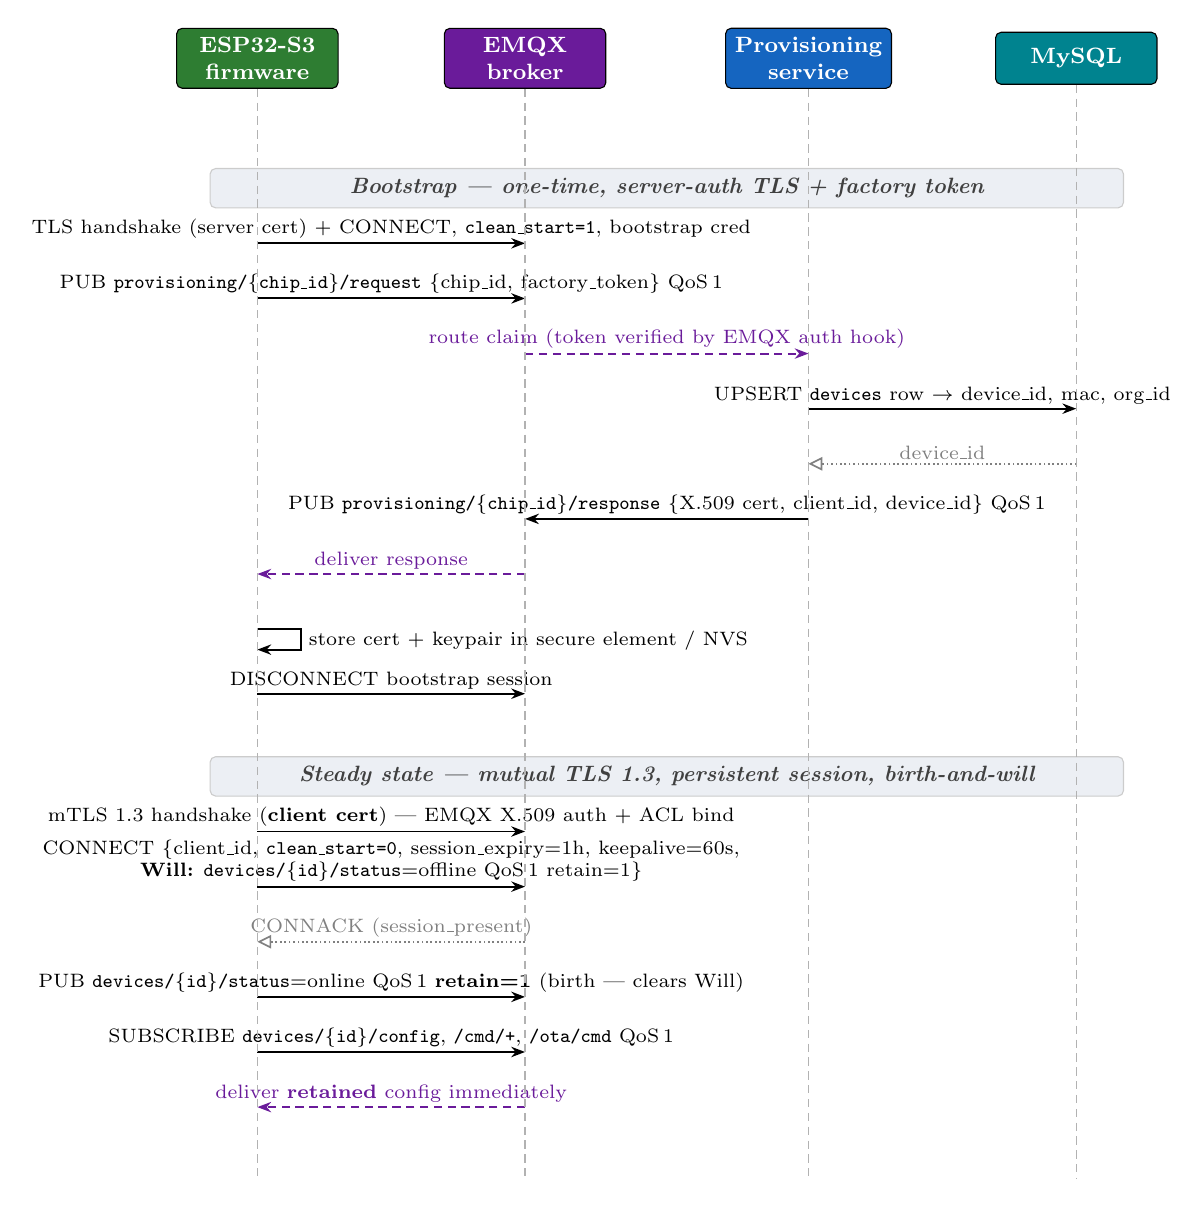
\begin{tikzpicture}
  \def\D{0}\def\B{3.4}\def\P{7.0}\def\M{10.4}
  \def\xmid{5.2}\def\bandw{11.6cm}
  \seqreset
  % headers
  \node[head, fill=devCol] (p0) at (\D,0) {ESP32-S3\\firmware};
  \node[head, fill=brkCol] (p1) at (\B,0) {EMQX\\broker};
  \node[head, fill=svcCol] (p2) at (\P,0) {Provisioning\\service};
  \node[head, fill=dbCol]  (p3) at (\M,0) {MySQL};

  \phase{Bootstrap — one-time, server-auth TLS + factory token}
  \mO{\D}{\B}{TLS handshake (server cert) + CONNECT, \texttt{clean\_start=1}, bootstrap cred}
  \mO{\D}{\B}{PUB \texttt{provisioning/\{chip\_id\}/request} \{chip\_id, factory\_token\} QoS\,1}
  \mA{\B}{\P}{route claim (token verified by EMQX auth hook)}
  \mO{\P}{\M}{UPSERT \texttt{devices} row $\rightarrow$ device\_id, mac, org\_id}
  \mR{\M}{\P}{device\_id}
  \mO{\P}{\B}{PUB \texttt{provisioning/\{chip\_id\}/response} \{X.509 cert, client\_id, device\_id\} QoS\,1}
  \mA{\B}{\D}{deliver response}
  \mS{\D}{store cert + keypair in secure element / NVS}
  \mO{\D}{\B}{DISCONNECT bootstrap session}

  \phase{Steady state — mutual TLS 1.3, persistent session, birth-and-will}
  \mO{\D}{\B}{mTLS 1.3 handshake (\textbf{client cert}) — EMQX X.509 auth + ACL bind}
  \mO{\D}{\B}{CONNECT \{client\_id, \texttt{clean\_start=0}, session\_expiry=1h, keepalive=60s,\\ \textbf{Will:} \texttt{devices/\{id\}/status}=offline QoS\,1 retain=1\}}
  \mR{\B}{\D}{CONNACK (session\_present)}
  \mO{\D}{\B}{PUB \texttt{devices/\{id\}/status}=online QoS\,1 \textbf{retain=1} (birth — clears Will)}
  \mO{\D}{\B}{SUBSCRIBE \texttt{devices/\{id\}/config}, \texttt{/cmd/+}, \texttt{/ota/cmd} QoS\,1}
  \mA{\B}{\D}{deliver \textbf{retained} config immediately}

  % lifelines
  \pgfmathsetmacro{\YBOT}{\YY-0.2}
  \foreach \p in {p0,p1,p2,p3}{\draw[lifeline] (\p.south) -- (\p.south|-0,\YBOT);}
\end{tikzpicture}}
\caption{Phase A — provisioning rotates a factory token into a per-device certificate, then
the production session is established with mutual TLS, a persistent MQTT~5.0 session, and a
retained will/birth pair so presence is never stale.}
\end{figure}

% =====================================================================
\newpage
\section*{3\quad Phase B — Steady-state telemetry (corrected ingestion)}

\begin{figure}[H]
\centering
\resizebox{\textwidth}{!}{%
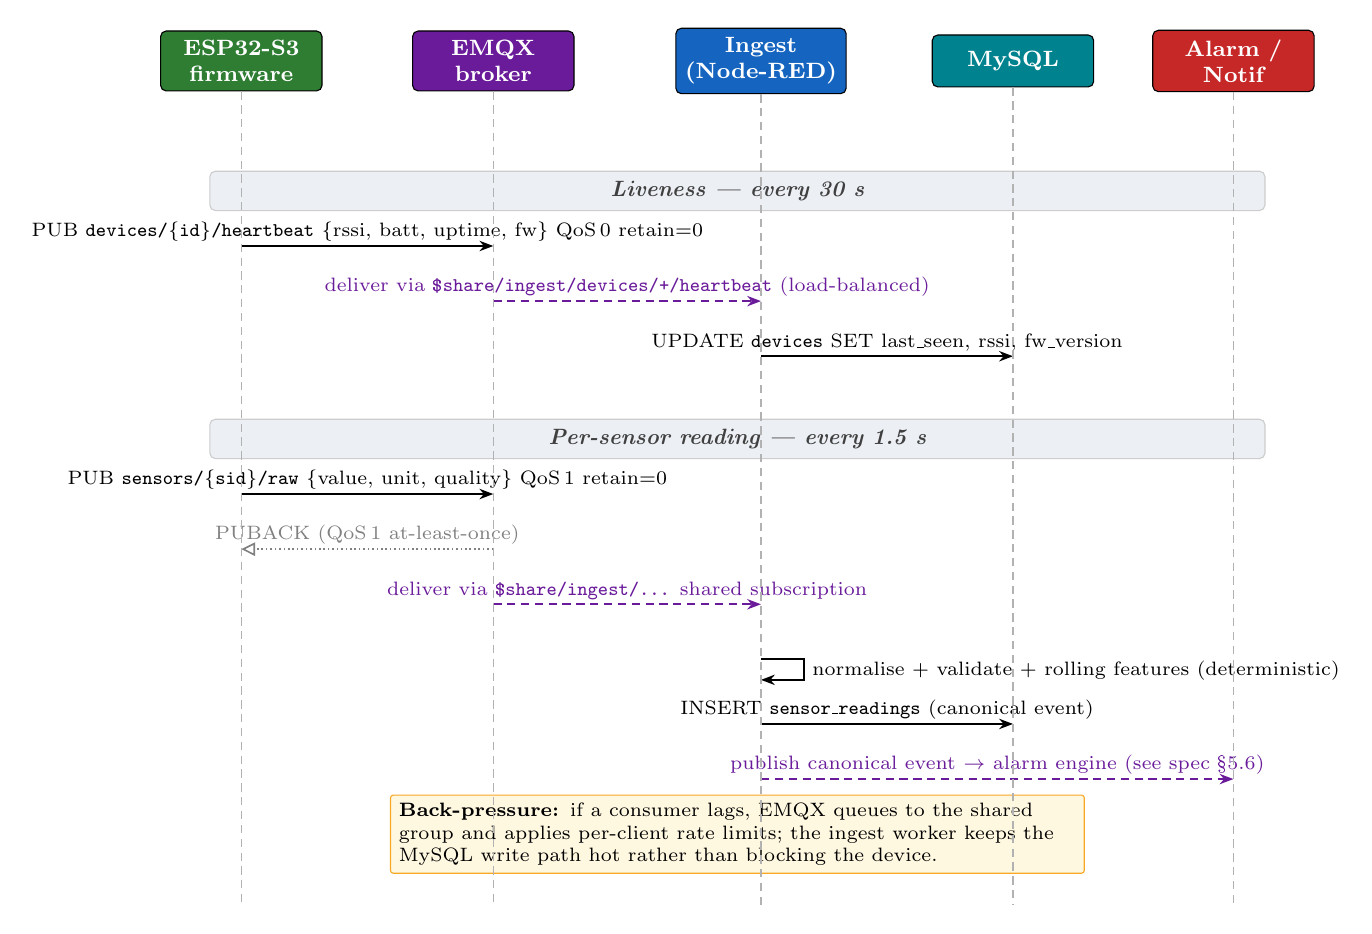
\begin{tikzpicture}
  \def\D{0}\def\B{3.2}\def\I{6.6}\def\M{9.8}\def\A{12.6}
  \def\xmid{6.3}\def\bandw{13.4cm}
  \seqreset
  \node[head, fill=devCol] (p0) at (\D,0) {ESP32-S3\\firmware};
  \node[head, fill=brkCol] (p1) at (\B,0) {EMQX\\broker};
  \node[head, fill=svcCol] (p2) at (\I,0) {Ingest\\(Node-RED)};
  \node[head, fill=dbCol]  (p3) at (\M,0) {MySQL};
  \node[head, fill=usrCol] (p4) at (\A,0) {Alarm /\\Notif};

  \phase{Liveness — every 30 s}
  \mO{\D}{\B}{PUB \texttt{devices/\{id\}/heartbeat} \{rssi, batt, uptime, fw\} QoS\,0 retain=0}
  \mA{\B}{\I}{deliver via \texttt{\$share/ingest/devices/+/heartbeat} (load-balanced)}
  \mO{\I}{\M}{UPDATE \texttt{devices} SET last\_seen, rssi, fw\_version}

  \phase{Per-sensor reading — every 1.5 s}
  \mO{\D}{\B}{PUB \texttt{sensors/\{sid\}/raw} \{value, unit, quality\} QoS\,1 retain=0}
  \mR{\B}{\D}{PUBACK (QoS\,1 at-least-once)}
  \mA{\B}{\I}{deliver via \texttt{\$share/ingest/\dots} shared subscription}
  \mS{\I}{normalise + validate + rolling features (deterministic)}
  \mO{\I}{\M}{INSERT \texttt{sensor\_readings} (canonical event)}
  \mA{\I}{\A}{publish canonical event $\rightarrow$ alarm engine (see spec \S5.6)}

  \note{6.3}{8.6cm}{\textbf{Back-pressure:} if a consumer lags, EMQX queues to the shared
  group and applies per-client rate limits; the ingest worker keeps the MySQL write path
  hot rather than blocking the device.}

  \pgfmathsetmacro{\YBOT}{\YY-0.2}
  \foreach \p in {p0,p1,p2,p3,p4}{\draw[lifeline] (\p.south) -- (\p.south|-0,\YBOT);}
\end{tikzpicture}}
\caption{Phase B — heartbeats stay QoS~0; sensor readings stay QoS~1 with PUBACK. The single
correction that matters for scale is consuming through an EMQX \emph{shared subscription},
which load-balances across ingest replicas and gives the broker a place to absorb back-pressure.}
\end{figure}

% =====================================================================
\newpage
\section*{4\quad Phase C — Signed OTA update with A/B rollback}

\begin{figure}[H]
\centering
\resizebox{\textwidth}{!}{%
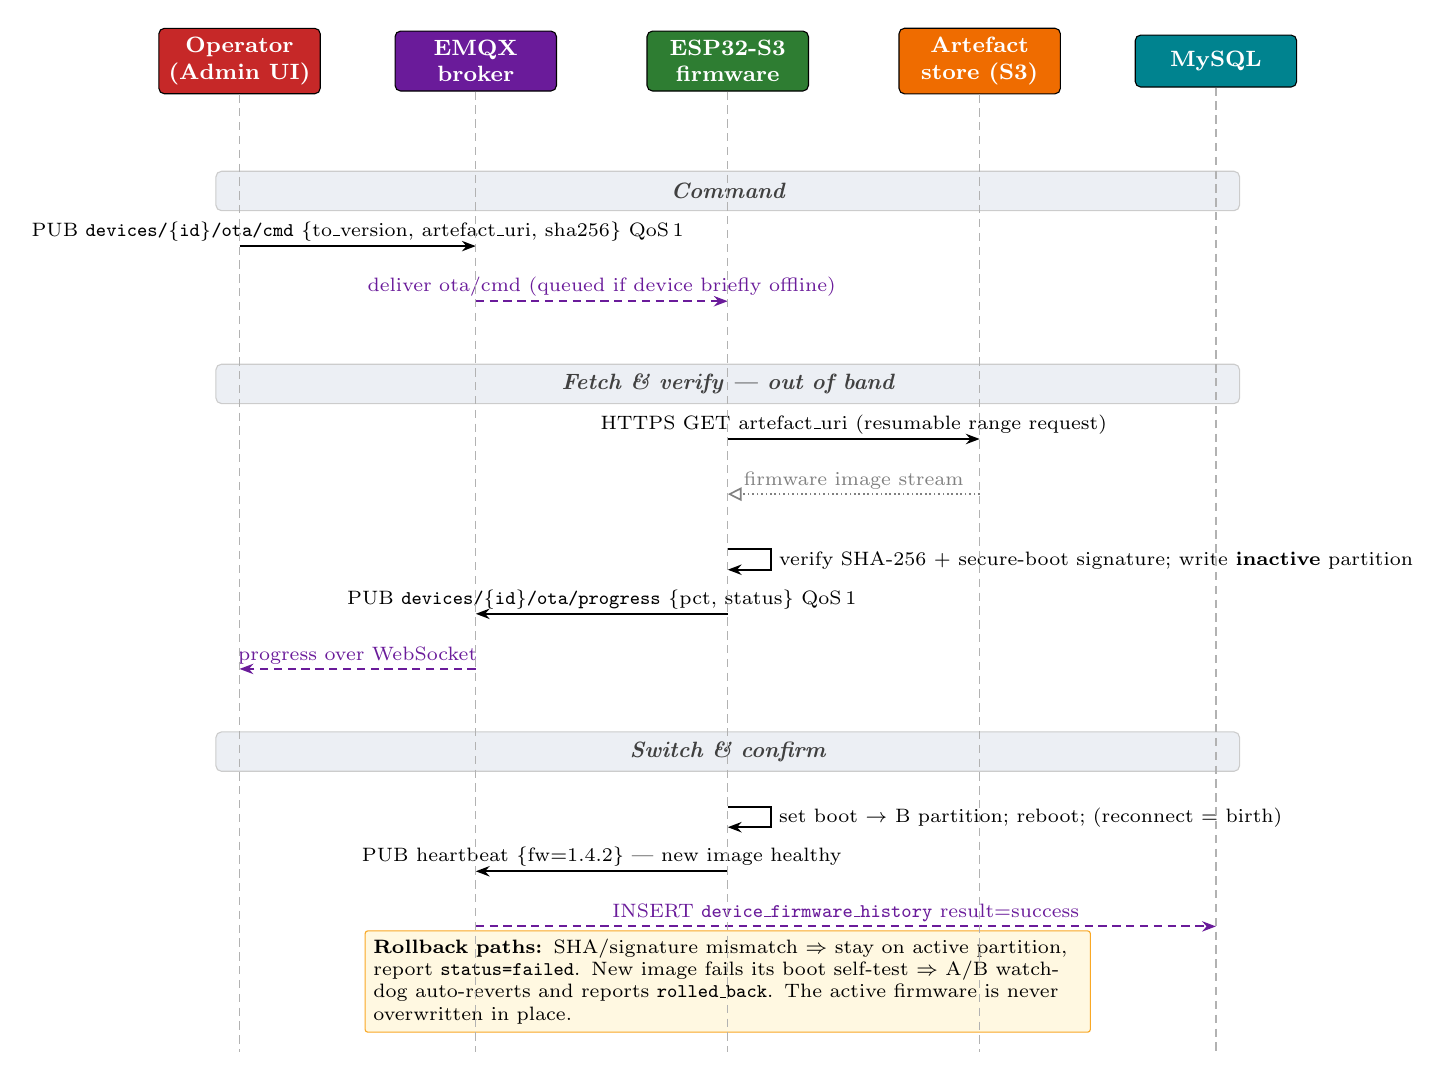
\begin{tikzpicture}
  \def\U{0}\def\B{3.0}\def\D{6.2}\def\O{9.4}\def\M{12.4}
  \def\xmid{6.2}\def\bandw{13.0cm}
  \seqreset
  \node[head, fill=usrCol] (p0) at (\U,0) {Operator\\(Admin UI)};
  \node[head, fill=brkCol] (p1) at (\B,0) {EMQX\\broker};
  \node[head, fill=devCol] (p2) at (\D,0) {ESP32-S3\\firmware};
  \node[head, fill=otaCol] (p3) at (\O,0) {Artefact\\store (S3)};
  \node[head, fill=dbCol]  (p4) at (\M,0) {MySQL};

  \phase{Command}
  \mO{\U}{\B}{PUB \texttt{devices/\{id\}/ota/cmd} \{to\_version, artefact\_uri, sha256\} QoS\,1}
  \mA{\B}{\D}{deliver ota/cmd (queued if device briefly offline)}

  \phase{Fetch \& verify — out of band}
  \mO{\D}{\O}{HTTPS GET artefact\_uri (resumable range request)}
  \mR{\O}{\D}{firmware image stream}
  \mS{\D}{verify SHA-256 + secure-boot signature; write \textbf{inactive} partition}
  \mO{\D}{\B}{PUB \texttt{devices/\{id\}/ota/progress} \{pct, status\} QoS\,1}
  \mA{\B}{\U}{progress over WebSocket}

  \phase{Switch \& confirm}
  \mS{\D}{set boot $\rightarrow$ B partition; reboot; (reconnect = birth)}
  \mO{\D}{\B}{PUB heartbeat \{fw=1.4.2\} — new image healthy}
  \mA{\B}{\M}{INSERT \texttt{device\_firmware\_history} result=success}

  \note{6.2}{9.0cm}{\textbf{Rollback paths:} SHA/signature mismatch $\Rightarrow$ stay on
  active partition, report \texttt{status=failed}. New image fails its boot self-test
  $\Rightarrow$ A/B watchdog auto-reverts and reports \texttt{rolled\_back}. The active
  firmware is never overwritten in place.}

  \pgfmathsetmacro{\YBOT}{\YY-0.2}
  \foreach \p in {p0,p1,p2,p3,p4}{\draw[lifeline] (\p.south) -- (\p.south|-0,\YBOT);}
\end{tikzpicture}}
\caption{Phase C — OTA is delivered as a signed artefact fetched out of band over HTTPS,
flashed to the inactive A/B slot, and only promoted after verification; the firmware
version reported in the next heartbeat closes the audit loop.}
\end{figure}

% =====================================================================
\section*{5\quad Phase D — Ungraceful disconnect (Last Will \& Testament)}

\begin{figure}[H]
\centering
\resizebox{0.92\textwidth}{!}{%
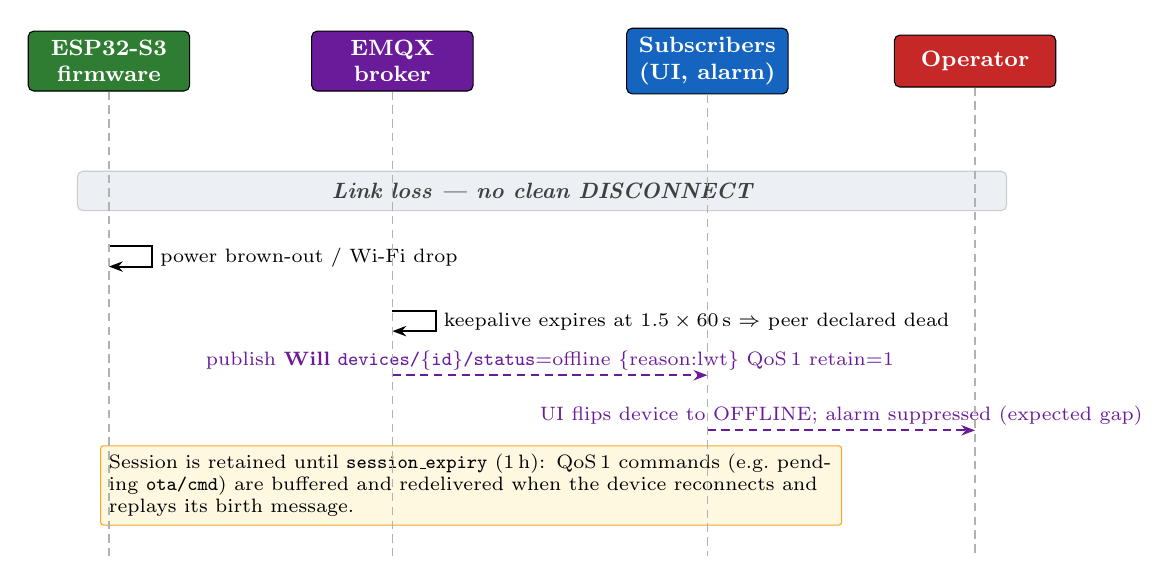
\begin{tikzpicture}
  \def\D{0}\def\B{3.6}\def\S{7.6}\def\U{11.0}
  \def\xmid{5.5}\def\bandw{11.8cm}
  \seqreset
  \node[head, fill=devCol] (p0) at (\D,0) {ESP32-S3\\firmware};
  \node[head, fill=brkCol] (p1) at (\B,0) {EMQX\\broker};
  \node[head, fill=svcCol] (p2) at (\S,0) {Subscribers\\(UI, alarm)};
  \node[head, fill=usrCol] (p3) at (\U,0) {Operator};

  \phase{Link loss — no clean DISCONNECT}
  \mS{\D}{power brown-out / Wi-Fi drop}
  \mS{\B}{keepalive expires at $1.5\times60$\,s $\Rightarrow$ peer declared dead}
  \mA{\B}{\S}{publish \textbf{Will} \texttt{devices/\{id\}/status}=offline \{reason:lwt\} QoS\,1 retain=1}
  \mA{\S}{\U}{UI flips device to OFFLINE; alarm suppressed (expected gap)}
  \note{4.6}{9.2cm}{Session is retained until \texttt{session\_expiry} (1\,h): QoS\,1 commands
  (e.g.\ pending \texttt{ota/cmd}) are buffered and redelivered when the device reconnects
  and replays its birth message.}

  \pgfmathsetmacro{\YBOT}{\YY-0.2}
  \foreach \p in {p0,p1,p2,p3}{\draw[lifeline] (\p.south) -- (\p.south|-0,\YBOT);}
\end{tikzpicture}}
\caption{Phase D — because the Will is registered at CONNECT with retain=1, presence stays
correct without any device cooperation; the retained session keeps queued commands alive
across the outage.}
\end{figure}

% =====================================================================
\section*{6\quad MQTT topic \& QoS contract (corrected)}
\begin{center}
\renewcommand{\arraystretch}{1.25}
\small
\begin{tabularx}{\textwidth}{@{}l c c c X@{}}
\toprule
\textbf{Topic} & \textbf{Dir} & \textbf{QoS} & \textbf{Retain} & \textbf{Notes} \\
\midrule
\texttt{provisioning/\{chip\_id\}/request}  & D$\to$B & 1 & 0 & bootstrap listener only \\
\texttt{provisioning/\{chip\_id\}/response} & B$\to$D & 1 & 0 & returns X.509 cert + client\_id \\
\texttt{devices/\{id\}/status}              & D$\to$B & 1 & \textbf{1} & Will \emph{and} birth on this topic \\
\texttt{devices/\{id\}/heartbeat}           & D$\to$B & 0 & 0 & 30\,s; liveness \& fw\_version \\
\texttt{sensors/\{sid\}/raw}                & D$\to$B & 1 & 0 & consumed via \texttt{\$share/ingest/} \\
\texttt{devices/\{id\}/config}              & B$\to$D & 1 & \textbf{1} & retained so it is read on subscribe \\
\texttt{devices/\{id\}/cmd/\{op\}}          & B$\to$D & 1 & 0 & reboot / calibrate / set-threshold \\
\texttt{devices/\{id\}/ota/cmd}             & B$\to$D & 1 & 0 & signed artefact descriptor \\
\texttt{devices/\{id\}/ota/progress}        & D$\to$B & 1 & 0 & percent + status \\
\bottomrule
\end{tabularx}
\end{center}

\paragraph{EMQX configuration checklist.}
\begin{itemize}[leftmargin=1.4em,itemsep=1pt]
  \item Dedicated TLS listeners: a \emph{bootstrap} listener (server-auth, token) and a
        \emph{production} listener (mutual TLS, \texttt{verify=verify\_peer},
        \texttt{fail\_if\_no\_peer\_cert=true}).
  \item Authentication chain: X.509 CN $\rightarrow$ \texttt{client\_id}; reject mismatched
        or duplicate client IDs.
  \item Authorization (ACL) pinned to \texttt{\$\{clientid\}} so each device is boxed into
        its own \texttt{devices/\{id\}/\#} and \texttt{sensors/\{sid\}/raw}.
  \item Shared subscriptions (\texttt{\$share/ingest/\dots}) for every server-side consumer;
        never a single static subscriber.
  \item Flapping detection + per-client rate \& bandwidth limits enabled.
  \item Session expiry sized to the longest tolerable command-delivery gap (here 1\,h).
\end{itemize}

\end{document}
